\documentclass[titlepage]{jsarticle}
\usepackage[dvipdfmx]{graphicx}
\usepackage{amsmath}
\usepackage{amssymb}
\usepackage{amsfonts}
\usepackage{comment}
\usepackage{h31ec-exp}
\usepackage{listings}
\usepackage{cases}
\lstset{
    basicstyle={\ttfamily},
    identifierstyle={\small},
    commentstyle={\smallitshape},
    keywordstyle={\small\bfseries},
    ndkeywordstyle={\small},
    stringstyle={\small\ttfamily},
    frame={tb},
    breaklines=true,
    columns=[l]{fullflexible},
    numbers=left,
    xrightmargin=0zw,
    xleftmargin=3zw,
    numberstyle={\scriptsize},
    stepnumber=1,
    numbersep=1zw,
    lineskip=-0.5ex,
    keepspaces=true,
    language=c
}
\renewcommand{\lstlistingname}{リスト}
\makeatletter
\newcommand{\figcaption}[1]{\def\@captype{figure}\caption{#1}}
\newcommand{\tblcaption}[1]{\def\@captype{table}\caption{#1}}
\makeatother

\title{OPアンプの基礎・応用}
\grade{4年32番}
\author{平田 蓮}
\team{}
\date{2020年12月11日}
\expdate{2020年11月19日, 11月26日, 12月3日, 12月10日}
\coauthor{
    30番 & 中川 太一 \\
    33番 & 藤田 悠生
}

\begin{document}
\maketitle
\section{目的}
    本実験では, アナログ回路の素子としてよく用いられるOPアンプを用いたアナログ
    回路の中から, 増幅回路, 演算回路取り上げ, その特性を理解することを目的とする.

    まず, 基本回路として反転増幅回路の特性を理解する.
    次に, 反転増幅回路を基本とした演算増幅回路として,
    微分回路, 積分回路を取り上げる. さらに応用回路として,
    信号に含まれる特定の周波数成分を取り出すフィルタ回路を設計し,
    その周波数特性を測定する.

\section{OPアンプの基本動作}
    OPアンプについて, 詳しくは実験テキスト\cite{text}
    に載っているためここでは代表的な特徴のみ示す.

    \begin{itemize}
        \item 閉ループ利得が非常に大きい(理想的には無限大)
        \item 入力インピーダンスが非常に大きい(理想的には無限大)
        \item 出力インピーダンスが低い(理想的には$0 \ \Omega$)
    \end{itemize}

    OPアンプをアナログ回路に利用する際は負帰還回路として用いることが多い.
    今回扱う回路も全て負帰還の回路である.

\section{使用機器}
    今回の使用機器を以下に示す.

    \begin{description}
        \item[OPアンプ] OP07
        \item[ブレッドボード] EC-12
        \item[直流電源] 
        \item[ファンクションジェネレータ] Ec-05
        \item[オシロスコープ] No.19
    \end{description}

\section{反転増幅回路}
    図\ref{fig:inv-amp}に反転増幅回路を示す.
    今回, 各素子の値は$R_i = 10\rm{k\Omega}$,
    $R_f = 20\rm{k\Omega}$である.

    \begin{figure}[h]
        \centering
        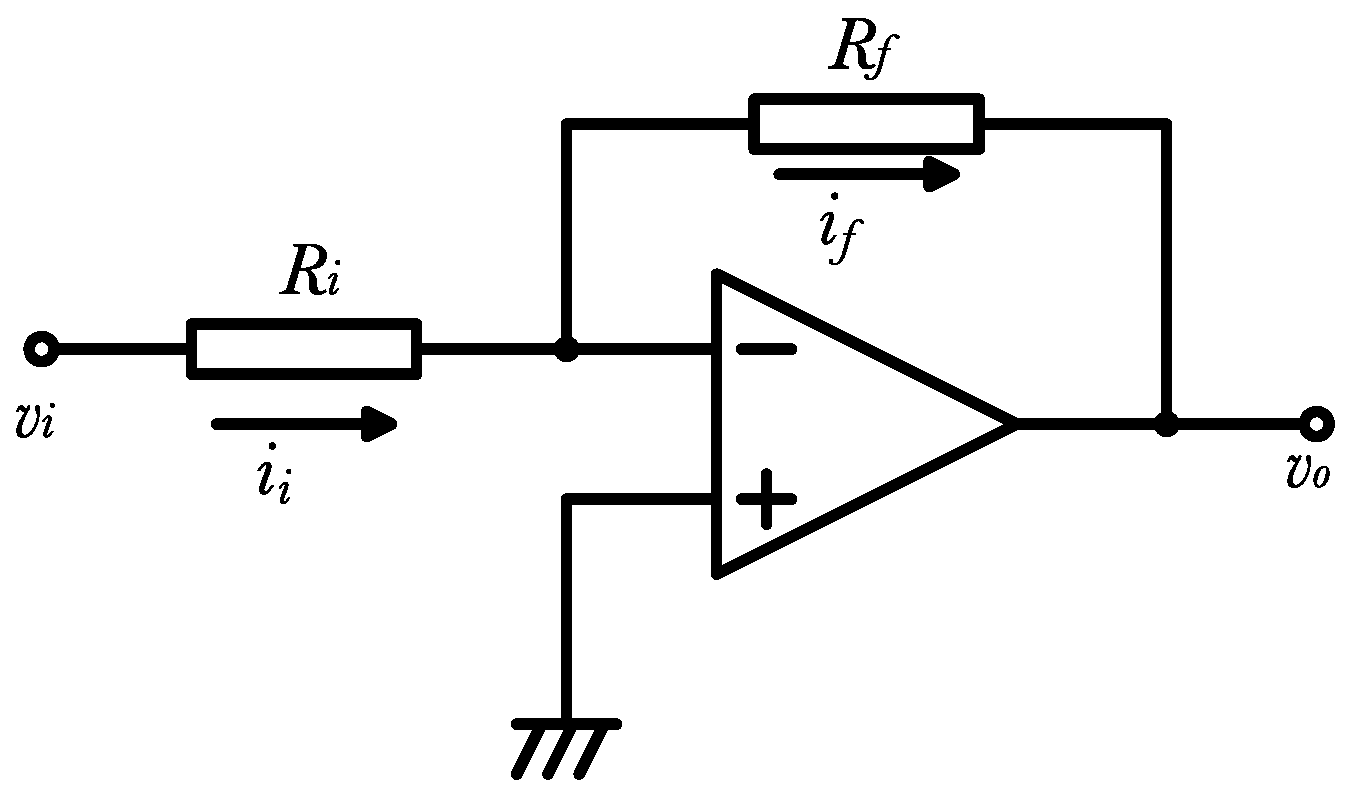
\includegraphics[width=0.7\hsize]{img/inv-amp.eps}
        \caption{反転増幅回路}
        \label{fig:inv-amp}
    \end{figure}

    この回路について, 閉ループ利得$A \ [倍]$, $G \ [\rm{dB}]$を求める.
    OPアンプの性質より, 二つの入力電圧を$v_s$とするとこれらは等しくなるので,
    二つの抵抗を流れる電流$i_i, i_f$について以下の式が成り立つ.

    \begin{equation}
        i_i = \frac{v_i - v_s}{R_i} = i_f = \frac{v_s - v_o}{R_f} \label{equ:inv-amp1}
    \end{equation}

    ここで, 理想的なOPアンプでの開ループ利得を$A_0 \rightarrow \infty$とすると,
    $\displaystyle v_s = \frac{v_o}{A_0} = 0$となるので,

    \begin{equation}
        \frac{v_i}{R_i} = -\frac{v_o}{R_f} \label{equ:inv-amp}
    \end{equation}

    となる. よって, 閉ループ利得は,

    \begin{eqnarray}
        A &=& \left|\frac{v_o}{v_i}\right| = \frac{R_f}{R_i} \nonumber \\
        G &=& 20 \log_{10}A \nonumber
    \end{eqnarray}

    と表せる.

    \subsection{周波数特性の測定} \label{sec:ex1}
        図\ref{fig:inv-amp}の回路に振幅2V,
        周波数$f = 100 \rm{Hz} \ 〜 \ 500 \rm{kHz}$の正弦波を入力し,
        出力波形のピークピーク値$V_o \ [\rm{V}]$及び
        入力波形に対する出力波形の遅れ$t \ [\mu\rm{s}]$を測定する.

        次に,測定結果をもとに, 閉ループ利得$G \ [\rm{dB}]$及び,
        出力波形の位相の遅れ$\displaystyle\phi = 360ft \ [^\circ]$を計算する.
        表\ref{tab:inv-amp}に測定結果及び計算結果を示す.

        \begin{table}[h]
            \caption{各周波数に対する出力波形の振幅と, 入力に対する遅れ}
            \label{tab:inv-amp}
            \centering
            \begin{tabular}{r|rr|rr||r|rr|rr}
                $f \ [\rm{kHz}]$ & $V_o \ [\rm{V]}$ & $G \ [\rm{dB}]$ & $t \ [\mu\rm{s}]$ & $\phi \ [^\circ]$ & $f \ [\rm{kHz}]$ & $V_o \ [\rm{V]}$ & $G \ [\rm{dB}]$ & $t \ [\mu\rm{s}]$ & $\phi \ [^\circ]$ \\ \hline \hline
                0.1 & 8.0 & 6.0 & 0 & 0 & 20 & 5.4 & 2.6 & 7.5 & -54 \\
                0.2 & 8.0 & 6.0 & 0 & 0 & 30 & 3.8 & -0.4 & 6.3 & -68 \\
                0.5 & 8.0 & 6.0 & 0 & 0 & 50 & 2.3 & -4.8 & 4.5 & -81 \\
                1 & 8.0 & 6.0 & 0 & 0 & 100 & 1.1 & -11.2 & 2.5 & -90 \\
                2 & 8.0 & 6.0 & 0 & 0 & 200 & 0.5 & -18.1 & 1.4 & -101 \\
                5 & 8.0 & 6.0 & 0 & 0 & 300 & 0.3 & -21.4 & 1.1 & -119 \\
                10 & 8.0 & 6.0 & 0 & 0 & 500 & 0.2 & -26.0 & 0.8 & -135 \\
            \end{tabular}
        \end{table}

        この結果を片対数グラフにプロットしたものを図\ref{fig:inv-amp-graph}に示す.

        \begin{figure}[h]
            \centering
            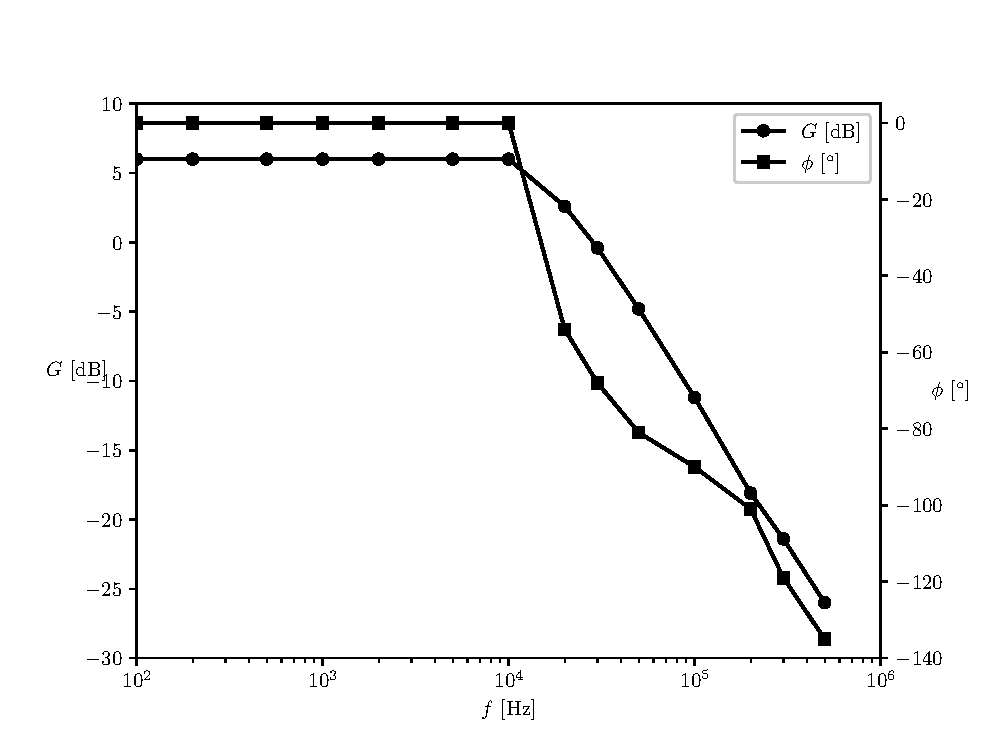
\includegraphics[width=0.8\hsize]{img/inv-amp-graph.eps}
            \caption{反転増幅回路の周波数特性}
            \label{fig:inv-amp-graph}
        \end{figure}

        グラフより,
        ある周波数を境に増幅率が下がりはじめ,
        位相も遅れていることがわかる.
        理論上はどんな周波数においてもOPアンプの利得は減衰しないが,
        実際の回路では高周波入力に対してOPアンプの出力が間に合わず,
        遅延が発生しているため増幅率が低下してしまうと考えられる.
        これは利得の低下とともに出力が遅延していることからもわかる.

    \subsection{課題1}
        \paragraph{
            式\ref{equ:inv-amp}の導出において,
            $A_0 \rightarrow \infty$の仮定を設けたが,
            $A_0$を有限値とした場合の式を求めよ. \\
        }
            式\ref{equ:inv-amp1}に$\displaystyle v_s = \frac{v_o}{A_0}$を代入すると,

            \begin{eqnarray}
                && \frac{v_i - v_s}{R_i} = \frac{v_s - v_o}{R_f} \nonumber \\
                &\leftrightarrow& \frac{v_o}{v_i} = \frac{R_f A_0}{(A_0 - 1)R_i + R_f} \label{equ:inv-amp-ex}
            \end{eqnarray}

            となる.

        \paragraph{
            式\ref{equ:inv-amp-ex}を用いて,
            $A_0$が20\%低下した場合の閉ループ利得$G$の変化を計算せよ.
            ただし, 使用するOPアンプの開ループ利得を$A_0 = 200000$とする. \\
        }
            式\ref{equ:inv-amp-ex}に
            $R_i = 10 \rm{k\Omega}$, $R_f = 20\rm{k\Omega}$,
            $A_0 = 200000$を代入すると,
            $\displaystyle\frac{v_o}{v_i} \approx 1.99999$が得られる.
            $A_0$が20\%低下したとき, $A_0 = 160000$となる.
            これを代入すると,
            $\displaystyle\frac{v_o}{v_i} \approx 1.9999875$となる.

            よって, $G$の変化,
            $\displaystyle20\log_{10}\frac{1.99999}{1.9999875} \approx 1.1 \times 10^{-5} \rm{dB}$
            が得られる.
            これより, 十分大きい開ループ利得帯では閉ループ利得の変化がほぼ起こらないと考えられる.

        \paragraph{
            十分高い周波数領域ではOPアンプの利得は-20dB/decで減衰する.
            \ref{sec:ex1}節で求めた閉ループ利得の特性線図において,
            高周波数領域の利得の減少を-20dB/decの直線で近似し,
            利得一定の直線との交点の周波数を求めよ. \\
        }

            利得の周波数特性グラフに近似線を追加したものを図\ref{fig:inv-amp-ex}
            に示す.
            二本の波線の交点の周波数は約15kHzである.
            グラフより,
            約15kHzの点で利得は最大値から3dB下がっていることがわかる.

            \begin{figure}[h]
                \centering
                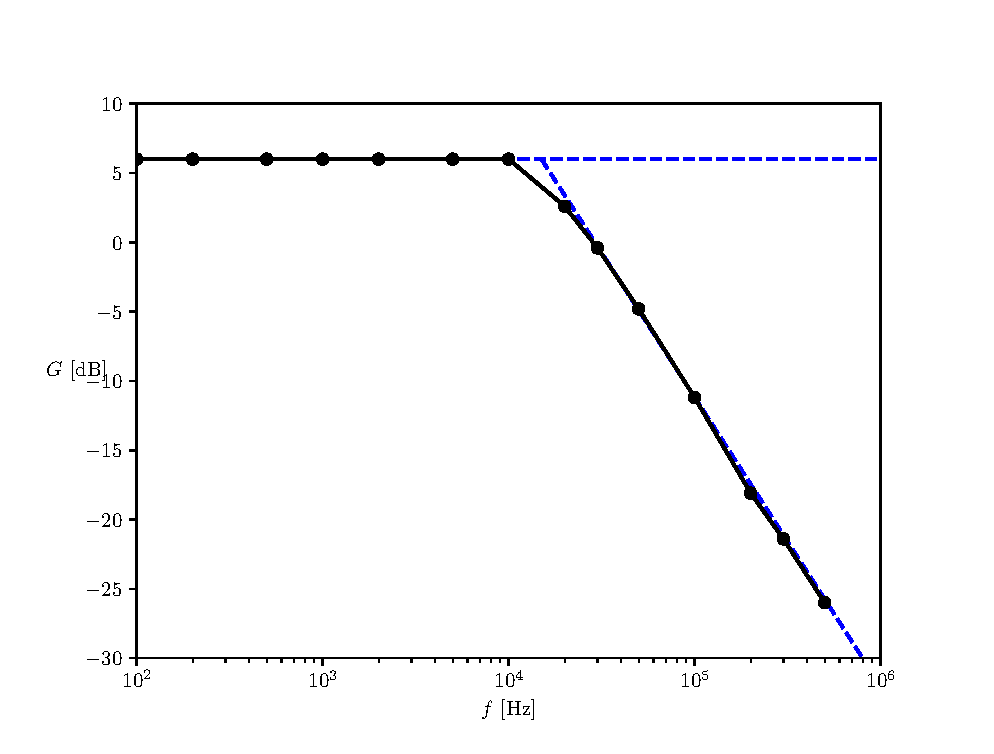
\includegraphics[width=0.8\hsize]{img/inv-amp-ex-graph.eps}
                \caption{利得の周波数特性の近似}
                \label{fig:inv-amp-ex}
            \end{figure}

\section{微分回路}
    微分回路は入力電圧の時間微分が出力電圧として得られる演算回路である.
    
    \subsection{基本微分回路}
        図\ref{fig:dif}に基本微分回路(BD)を示す.
        今回は, $R_f = 20\rm{k\Omega}$, $C = 0.0022\rm{\mu F}$とする.

        \begin{figure}[h]
            \centering
            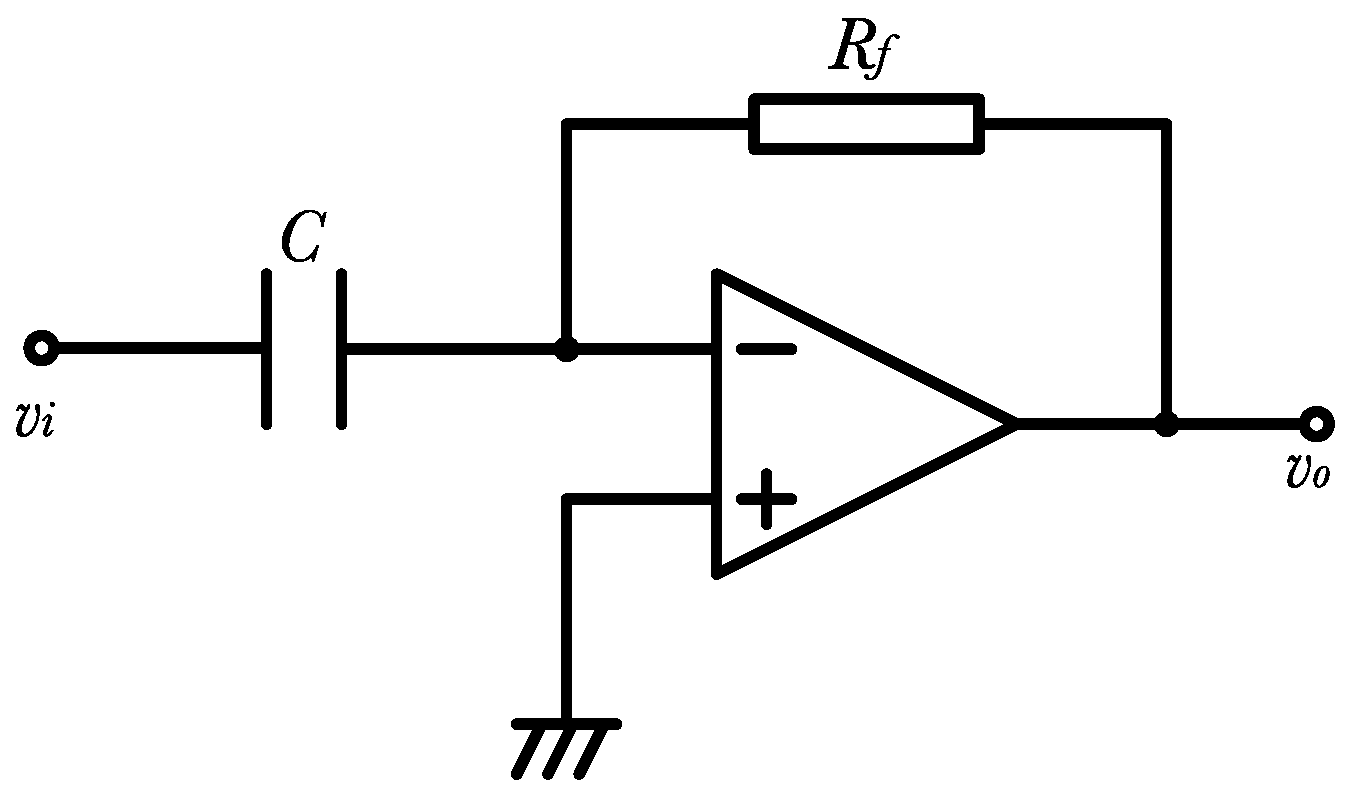
\includegraphics[width=0.7\hsize]{img/div.eps}
            \caption{基本微分回路}
            \label{fig:dif}
        \end{figure}

        この回路の入出力電圧$v_i$, $v_o$について
        $\displaystyle v_o = -CR_f\frac{dv_i}{dt}$
        が成り立つ.

        特に, 入力電圧を正弦波交流
        $v_i = -\omega CR_fV_m\sin(\omega t) \ (\omega = 2\pi f)$
        とすると,

        \begin{equation}
            v_o = -\omega CR_fV_m\cos(\omega t) \label{equ:dif}
        \end{equation}

        となる.
        これらの式の詳しい導出は実験テキスト\cite{text}に載っているため,
        省略する.

        \subsubsection{入出力波形の観察}
            基本微分回路に入力として以下の二つの波形を与えたときの出力電圧の
            波形を記録する.

            \begin{itemize}
                \item 正弦波 (振幅0.5V, 周波数1kHz)
                \item 矩形波 (振幅0.5V, 周波数1kHz)
            \end{itemize}

            正弦波を入力した際の入出力波形を図\ref{fig:dif1}に示す.

            \begin{figure}[h]
                \centering
                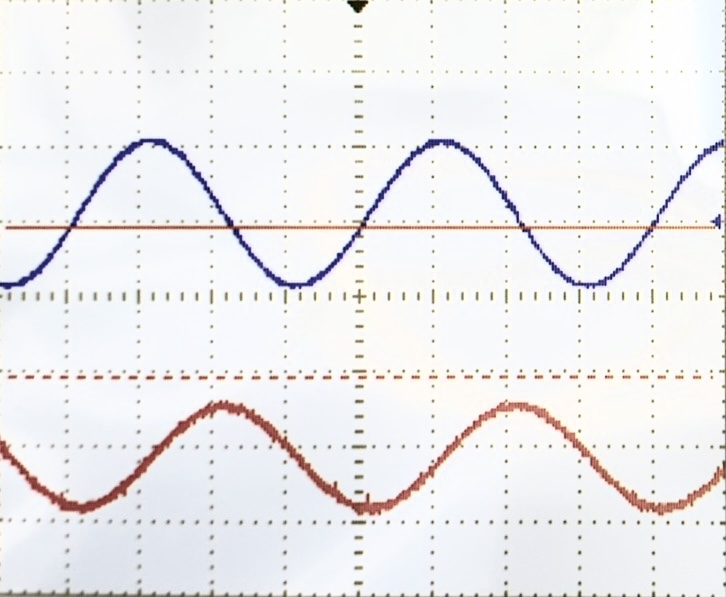
\includegraphics[width=10cm]{img/dif-graph1.jpg}
                \caption{基本微分回路に正弦波を入力した様子}
                \label{fig:dif1}
            \end{figure}

            上の波形が入力で, 下の波形が出力である.
            式\ref{equ:dif}に$\omega = 2000\pi \ \rm{rad/s}$,
            $R_f = 20 \rm{k\Omega}$, $C = 0.0022 \rm{\mu F}$,
            $V_m = 0.5 \rm{V}$
            を代入すると, $v_o \approx -0.138 \cos(6280t) \ \rm{[V]}$となる.
            入力は$\sin$であるので, 波形の位相差からも
            正しく波形が見れていることがわかる.

            次に, 図\ref{fig:dif2}に矩形波を入力した際の様子と,
            それを時間軸方向に拡大した図を示す.

            \begin{figure}[h]
                \begin{minipage}{0.5\hsize}
                    \centering
                    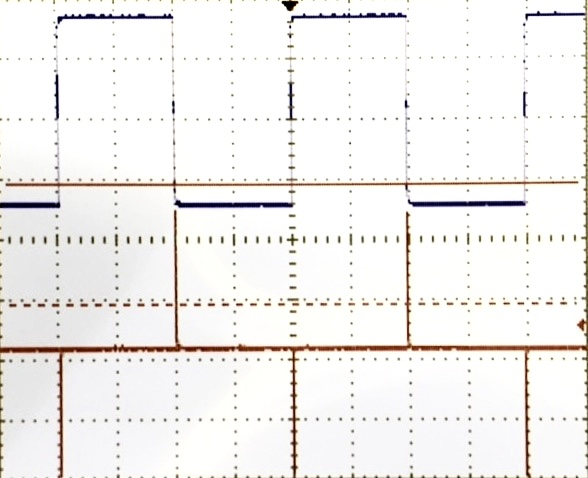
\includegraphics[width=8cm]{img/dif-graph2.jpg}
                \end{minipage}
                \begin{minipage}{0.5\hsize}
                    \centering
                    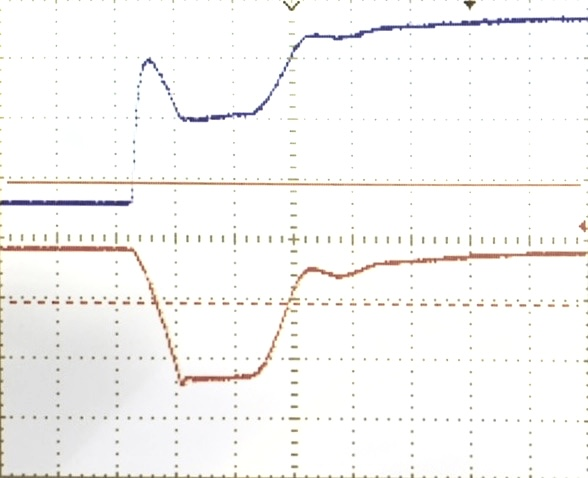
\includegraphics[width=8cm]{img/dif-graph3.jpg}
                \end{minipage}
                \caption{基本微分回路に矩形波を入力した様子}
                \label{fig:dif2}
            \end{figure}

            図を見ると,
            入出力ともに矩形波発生器の問題で
            波形に歪みが生じていることがわかる.

        \subsubsection{周波数特性の測定} \label{sec:ex2}
            \ref{sec:ex1}と同様に振幅0.5V,
            周波数100Hz〜20kHzの正弦波を入力して周波数特性を測定する.
            表\ref{tab:dif}に計算結果を示す.

            \begin{table}[h]
                \caption{各周波数に対する出力波形の振幅と, 入力に対する遅れ}
                \label{tab:dif}
                \centering
                \begin{tabular}{r|rr||r|rr}
                    $f \ [\rm{kHz}]$ & $G \ [\rm{dB}]$ & $\phi \ [^\circ]$ & $f \ [\rm{kHz}]$ & $G \ [\rm{dB}]$ & $\phi \ [^\circ]$ \\ \hline \hline
                    0.1 & -31.1 & -90.1 & 2 & -5.1 & -89.0 \\
                    0.2 & -25.0 & -90.2 & 5 & 2.8 & -91.9 \\
                    0.5 & -17.1 & -90.3 & 10 & 8.9 & -92.8 \\
                    1 & -11.1 & -90.5 & 20 & 15.1 & -93.6 \\
                \end{tabular}
            \end{table}

            表のデータをプロットしたものを図\ref{fig:difex1}に示す.

            \begin{figure}[h]
                \centering
                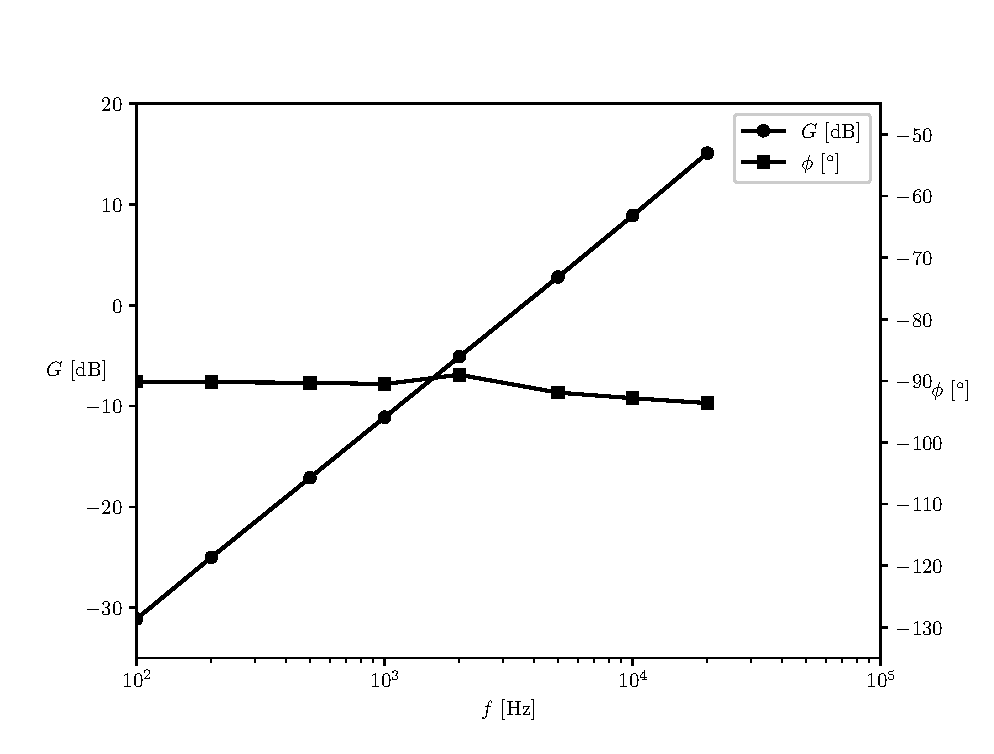
\includegraphics[width=0.8\hsize]{img/difex-graph1.eps}
                \caption{基本微分回路の周波数特性}
                \label{fig:difex1}
            \end{figure}

            図より, 周波数が上がるにつれて回路の利得が上がっていることがわかる.
            また, 入力に対する出力の位相の遅れは常に約 -90$^\circ$である.

    \subsection{実用微分回路}
        基本微分回路では, \ref{sec:ex2}節からも明らかなように,
        周波数の増加とともに出力電圧が無限大に増加してしまう.
        これを防ぐために抵抗$R_s$を追加した実用微分回路(PD)を
        \ref{fig:nice-dif}に示す.
        今回は各素子の値を
        $R_s = 10\rm{k\Omega}$, $R_f = 20\rm{k\Omega}$, $C = 0.0022\rm{\mu F}$とする.

        \begin{figure}[h]
            \centering
            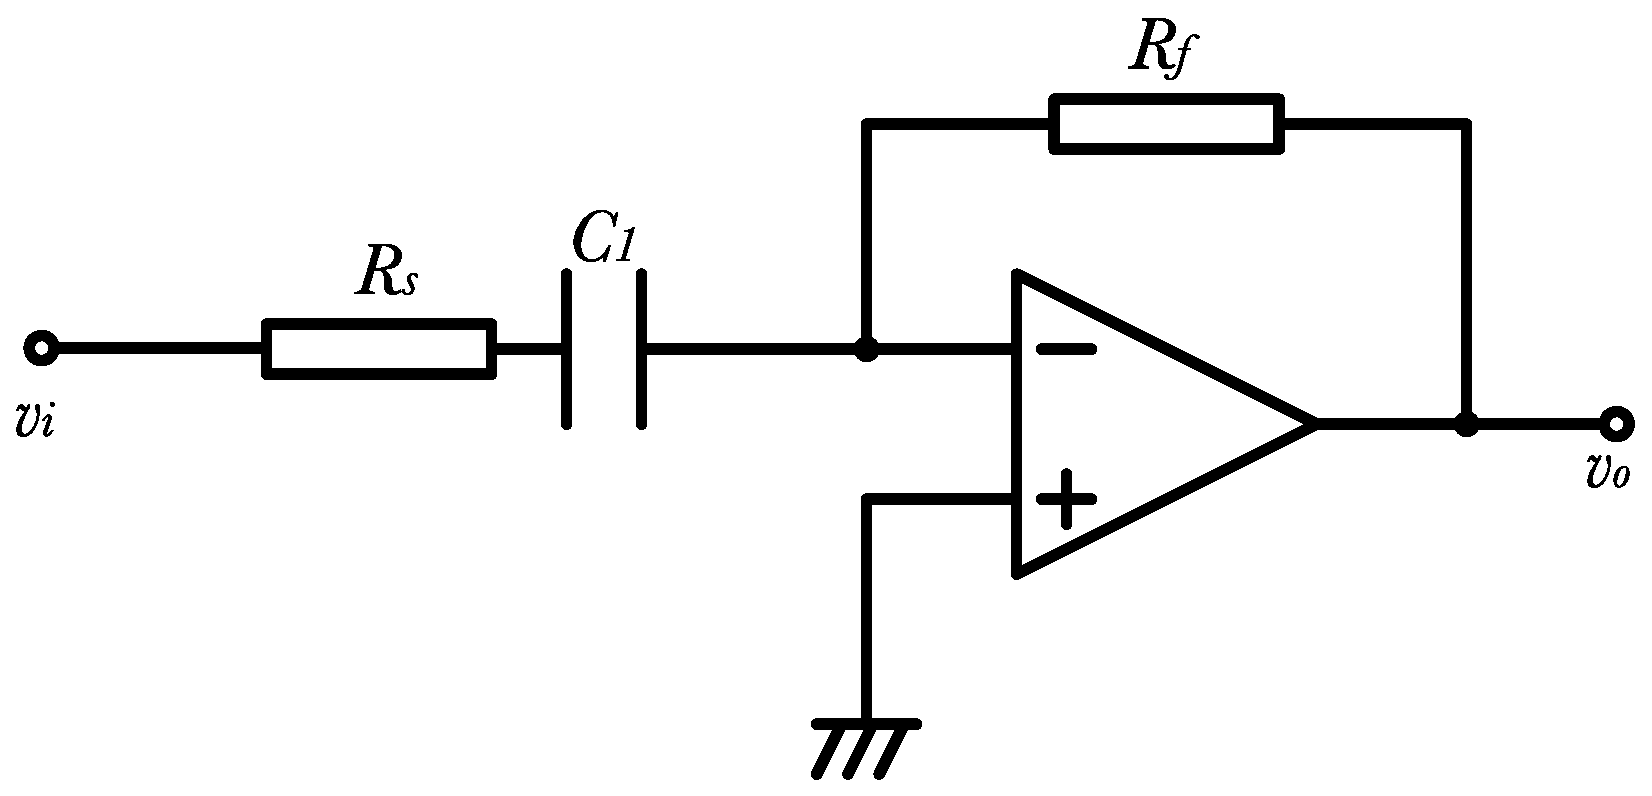
\includegraphics[width=0.7\hsize]{img/nice-dif.eps}
            \caption{実用微分回路}
            \label{fig:nice-dif}
        \end{figure}

        \subsubsection{周波数特性の測定} \label{sec:ex3}
            \ref{sec:ex1}, \ref{sec:ex2}と同様に振幅0.5V,
            周波数100Hz〜50kHzの正弦波を入力して周波数特性を測定する.
            表\ref{tab:nice-dif}に計算結果を示す.

            \begin{table}[h]
                \caption{各周波数に対する利得と, 入力に対する位相の遅れ}
                \label{tab:nice-dif}
                \centering
                \begin{tabular}{r|rr||r|rr}
                    $f \ [\rm{kHz}]$ & $G \ [\rm{dB}]$ & $\phi \ [^\circ]$ & $f \ [\rm{kHz}]$ & $G \ [\rm{dB}]$ & $\phi \ [^\circ]$ \\ \hline \hline
                    0.1 & -31.0 & -91.0 & 7 & 2.9 & -134.8 \\
                    0.2 & -24.9 & -91.8 & 8 & 3.4 & -138.5 \\
                    0.5 & -17.0 & -94.3 & 9 & 3.9 & -141.8 \\
                    1 & -11.0 & -98.3 & 10 & 4.2 & -144.6 \\
                    2 & -5.3 & -106.1 & 20 & 5.5 & -160.4 \\
                    5 & -1.2 & -125.5 & 50 & 5.9 & -171.8 \\
                \end{tabular}
            \end{table}

            表のデータをプロットしたものを図\ref{fig:nice-dif-graph},
            表\ref{tab:dif}, \ref{tab:nice-dif}のデータを合わせてプロットしたものを
            図\ref{fig:dif-com-graph}に示す.

            \begin{figure}[h]
                \centering
                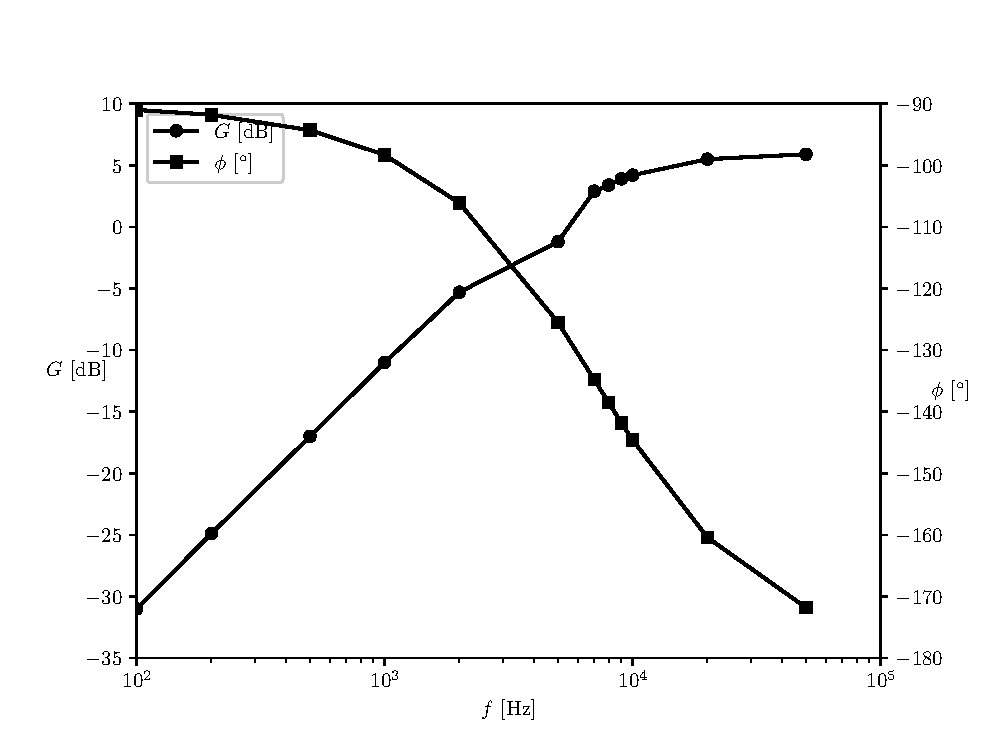
\includegraphics[width=0.8\hsize]{img/nice-dif-graph.eps}
                \caption{実用微分回路の周波数特性}
                \label{fig:nice-dif-graph}
            \end{figure}

            \begin{figure}[h]
                \begin{minipage}{0.5\hsize}
                    \centering
                    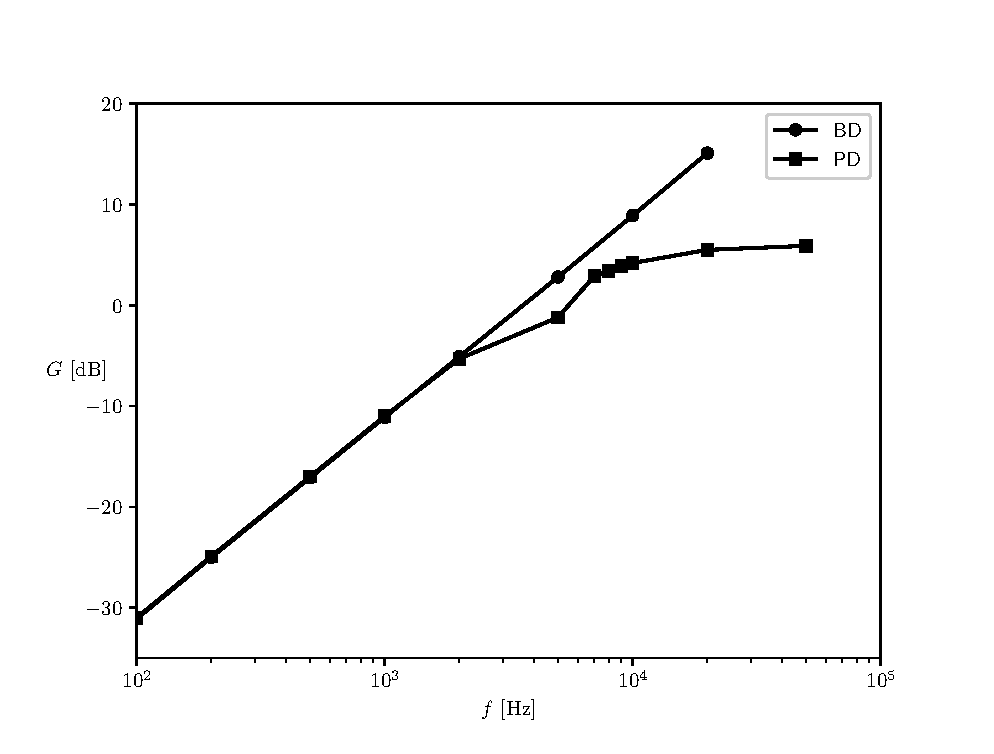
\includegraphics[width=1.1\hsize]{img/dif-com-graph1.eps}
                \end{minipage}
                \begin{minipage}{0.5\hsize}
                    \centering
                    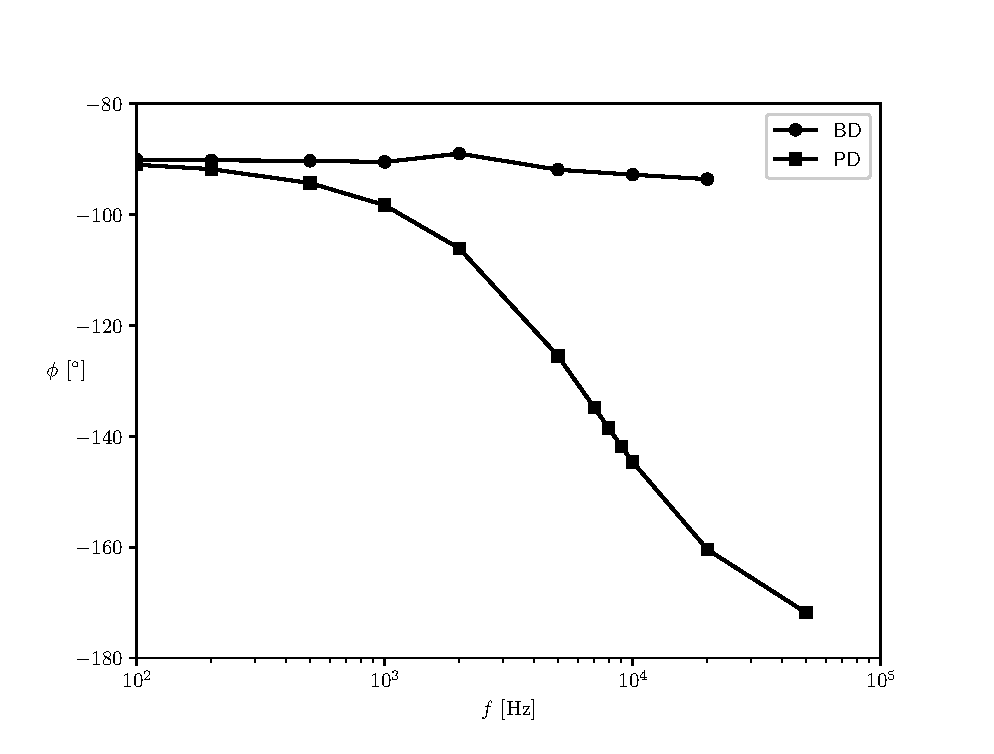
\includegraphics[width=1.1\hsize]{img/dif-com-graph2.eps}
                \end{minipage}
                \caption{周波数特性の比較}
                \label{fig:dif-com-graph}
            \end{figure}

            図より, 基本微分回路では周波数の上昇につれて
            出力が増加しているが,
            実用微分回路では一定値に収束している.
            また, それに伴い出力の位相も遅れていることがわかる.

    \subsection{課題2}
        \paragraph{実用微分回路の閉ループ利得と位相差を周波数の関数として具体的に求めよ. \\}
            図\ref{fig:nice-dif}より,
            次の式を立てられる.

            \begin{numcases}
                {}
                v_i(t) = i(t)\left(R_s - j\frac{1}{\omega C}\right) & \nonumber \\
                v_o(t) = -i(t)R_f & \nonumber
            \end{numcases}

            これらをラプラス変換して,

            \begin{numcases}
                {}
                V_i(s) = I(s)\left(R_s + \frac{1}{sC}\right) & \nonumber \\
                V_o(s) = -I(s)R_f & \nonumber
            \end{numcases}

            となる. よって$v_i$から$v_o$の伝達関数は,

            \begin{equation*}
                \frac{V_i(s)}{V_o(s)} = -\frac{R_f}{R_s + \frac{1}{sC}} = -\frac{sCR_f}{sCR_s + 1}
            \end{equation*}

            である. これに, $R_s = 10\rm{k\Omega}$, $R_f = 20\rm{k\Omega}$,
            $C = 0.0022\rm{\mu F}$を代入すると,
            $\displaystyle -\frac{0.000044s}{0.000022s + 1}$となる.
            これにさらに$s = j\omega$を代入すると
            $\displaystyle -\frac{j0.000044\omega}{1 + j0.000022\omega} = -\frac{j0.000088\pi f}{1 + j0.000044\pi f}$
            となり, 閉ループ利得を表す周波数の関数となる.

            また, これの偏角を求めると,
            $\displaystyle\phi = \arctan\frac{\frac{1}{\omega C}}{R_s} = \arctan\frac{1}{0.000044\pi f}$
            となる.

            これらの式を\ref{sec:ex3}の結果に重ねてプロットしたものを
            図\ref{fig:difex2}に示す.

            \begin{figure}[h]
                \begin{minipage}{0.5\hsize}
                    \centering
                    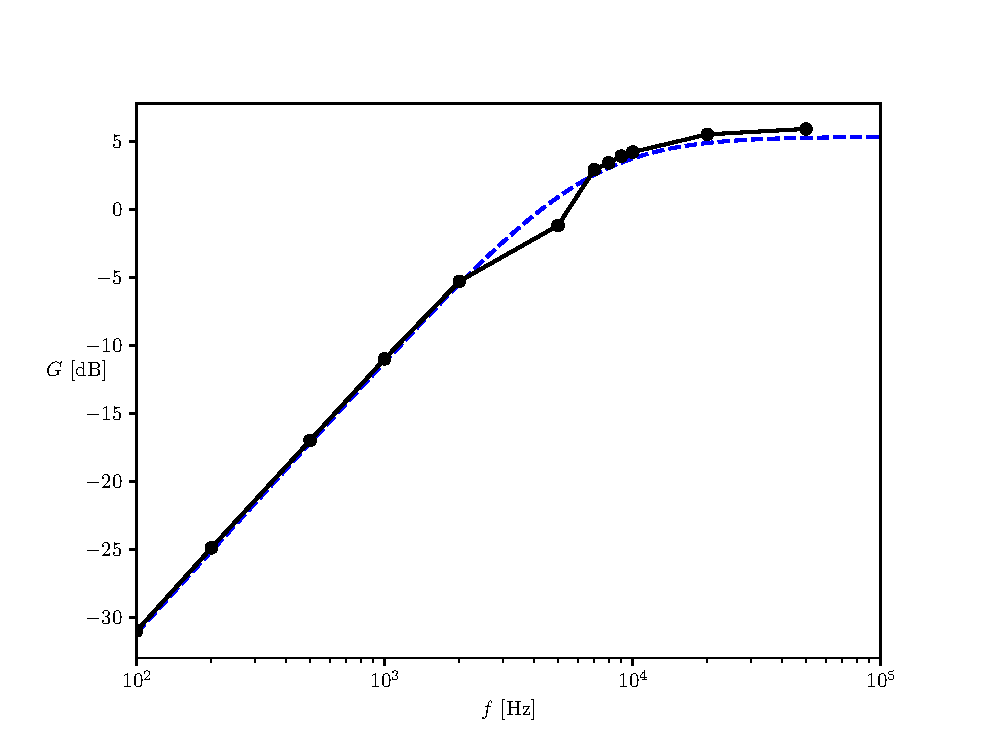
\includegraphics[width=1.1\hsize]{img/ex2-1.eps}
                \end{minipage}
                \begin{minipage}{0.5\hsize}
                    \centering
                    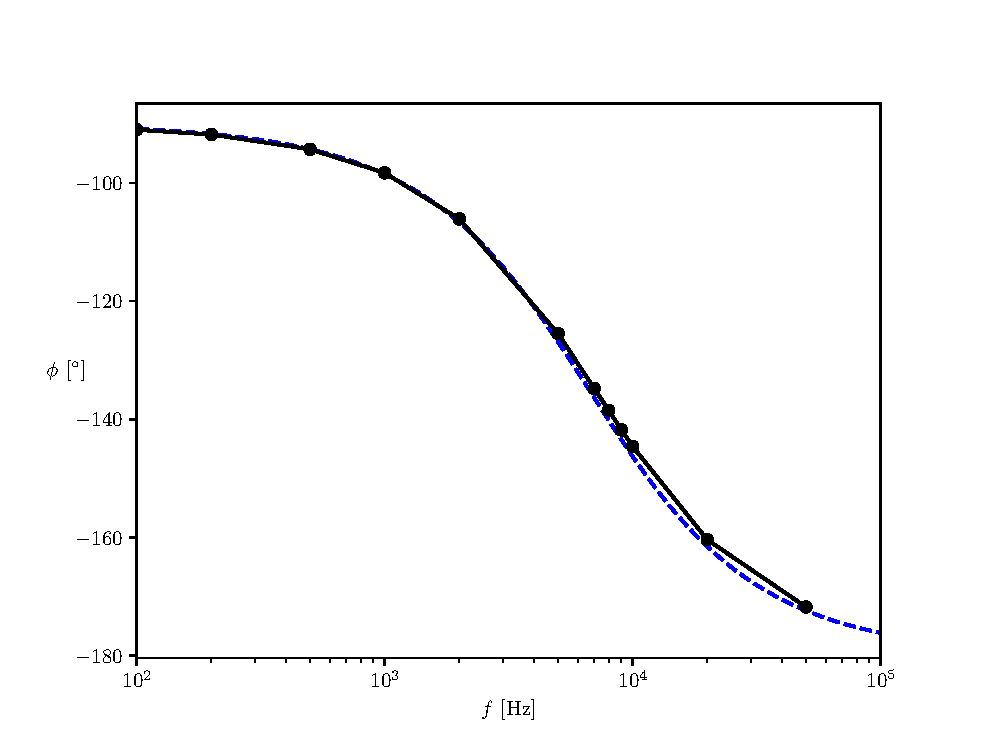
\includegraphics[width=1.1\hsize]{img/ex2-2.eps}
                \end{minipage}
                \caption{理論値と計測値の比較}
                \label{fig:difex2}
            \end{figure}
            
            図より実験が正しく行われていたことがわかる.

\section{積分回路}
    積分回路は微分回路とは逆に入力電圧の時間積分を出力する回路である.

    \subsection{基本積分回路}
        図\ref{fig:int}に基本積分回路(BI)を示す.
        今回は$R_1 = 10\rm{k\Omega}$, $C = 0.0022\rm{\mu F}$
        の素子を使う.

        \begin{figure}[h]
            \centering
            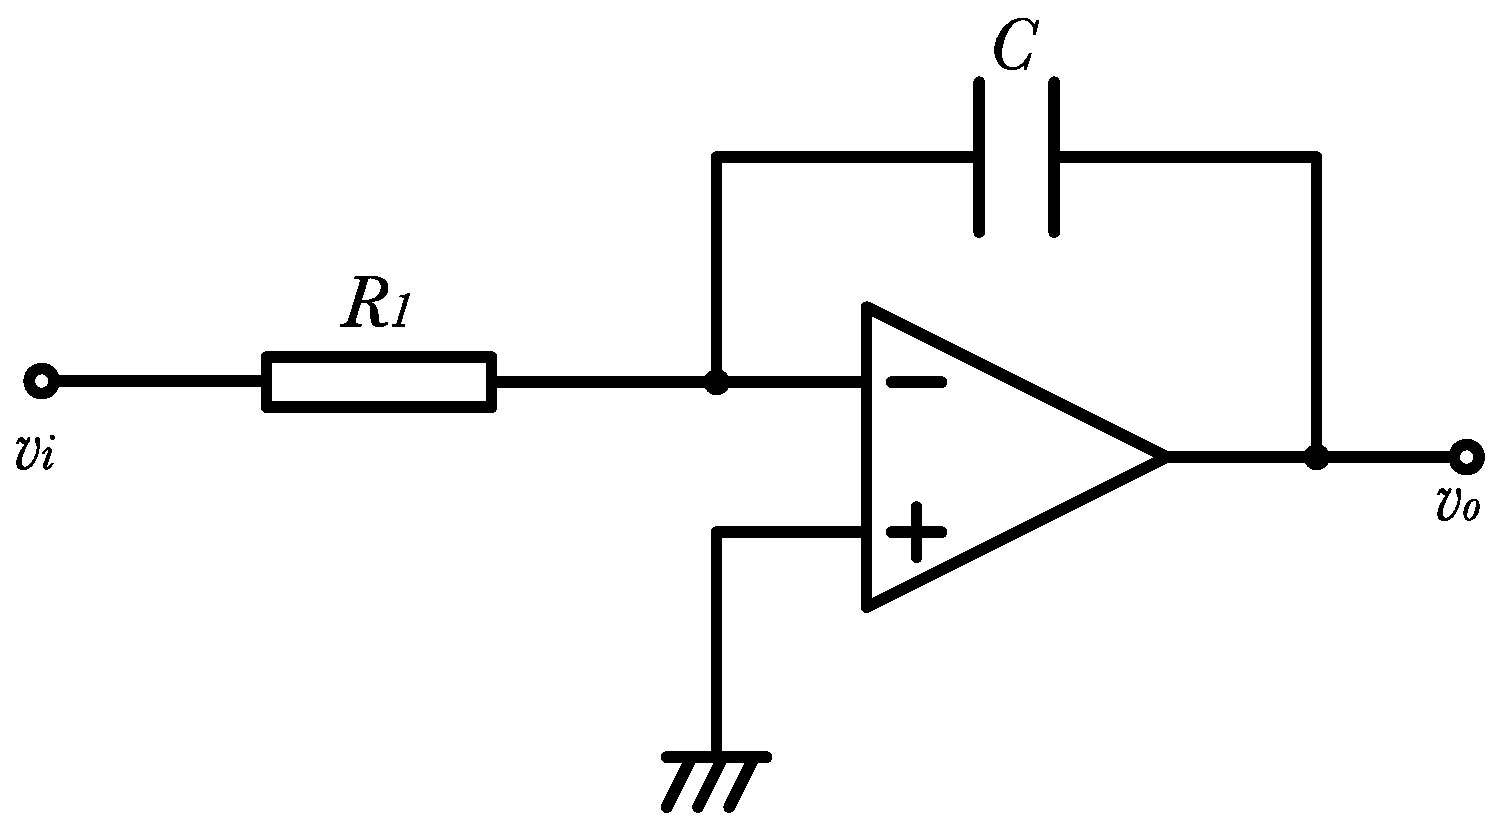
\includegraphics[width=0.7\hsize]{img/int.eps}
            \caption{基本積分回路}
            \label{fig:int}
        \end{figure}

        この回路の入出力電圧$v_i$, $v_o$について
        $\displaystyle v_o = -\frac{1}{R_1C}\int^t_0v_i(\tau)d\tau$
        が成り立つ.

        特に, 入力電圧を正弦波交流
        $v_i = V_m\sin(\omega t) \ (\omega = 2\pi f)$
        とすると,

        \begin{equation}
            v_o = \frac{V_m}{\omega R_1C}\cos(\omega t) \label{equ:int}
        \end{equation}

        となる.
        これらの式の詳しい導出は実験テキスト\cite{text}に載っているため,
        省略する.

        \subsubsection{入出力波形の観察}
            基本積分回路に入力として以下の二つの波形を与えたときの出力電圧の
            波形を記録する.

            \begin{itemize}
                \item 正弦波 (振幅0.5V, 周波数1kHz)
                \item 矩形波 (振幅0.5V, 周波数1kHz)
            \end{itemize}

            正弦波を入力した際の入出力波形を図\ref{fig:int1}に示す.

            \begin{figure}[h]
                \centering
                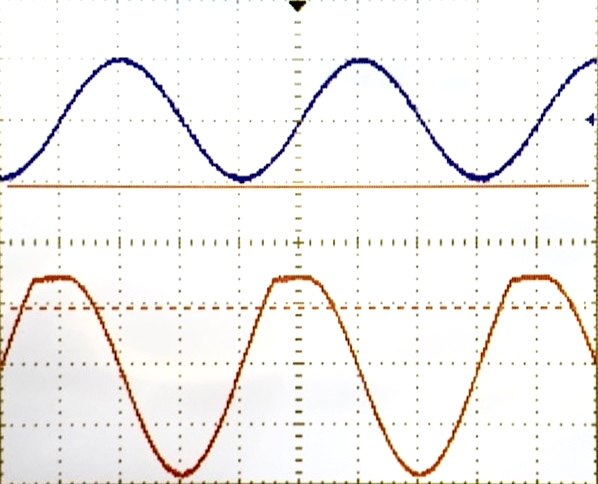
\includegraphics[width=10cm]{img/int-graph1.jpg}
                \caption{基本積分回路に正弦波を入力した様子}
                \label{fig:int1}
            \end{figure}

            上の波形が入力で, 下の波形が出力である.
            式\ref{equ:int}に$\omega = 2000\pi \ \rm{rad/s}$,
            $R_1 = 10 \rm{k\Omega}$, $C = 0.0022 \rm{\mu F}$,
            $V_m = 0.5 \rm{V}$
            を代入すると, $v_o \approx 3.62 \cos(6280t) \ \rm{[V]}$となる.
            入力は$\sin$であるので, 波形の位相差からも
            正しく波形が見れていることがわかる.

            次に, 図\ref{fig:int2}に矩形波を入力した際の様子を示す.

            \begin{figure}[h]
                \centering
                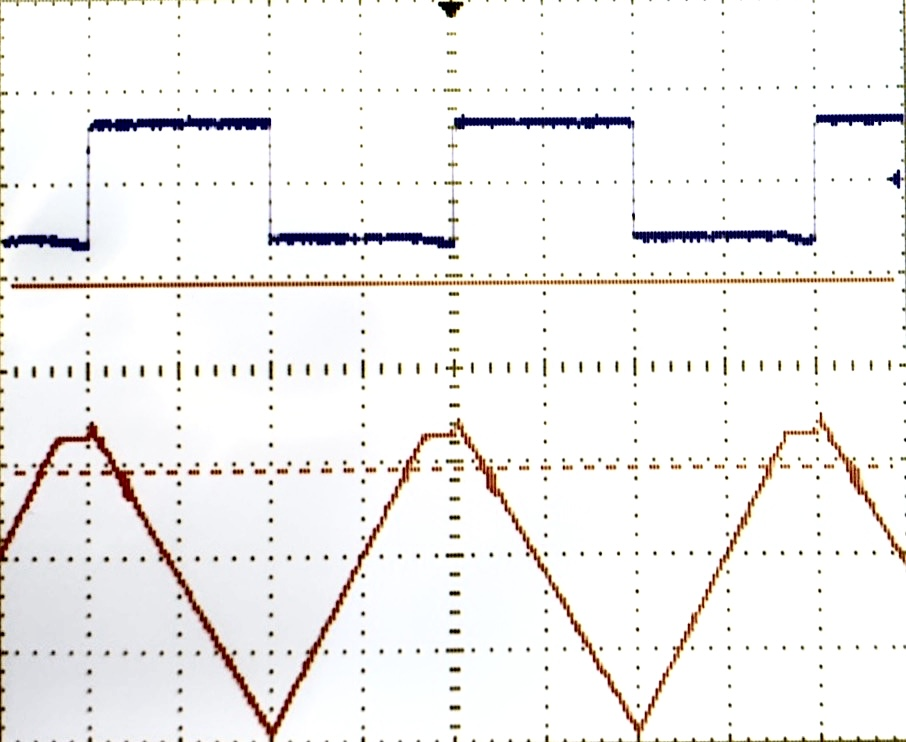
\includegraphics[width=10cm]{img/int-graph2.jpg}
                \caption{基本積分回路に矩形波を入力した様子}
                \label{fig:int2}
            \end{figure}

            回路の仕組み上,
            実際の積分値とは正負が逆転した出力が得られていることがわかる.

        \subsubsection{周波数特性の測定} \label{sec:ex4}
            基本積分回路に振幅0.5V,
            周波数300Hz〜50kHzの入力を与え,
            周波数特性を測定する.
            表\ref{tab:int}に計算結果を示す.

            \begin{table}[h]
                \caption{各周波数に対する出力波形の振幅と, 入力に対する遅れ}
                \label{tab:int}
                \centering
                \begin{tabular}{r|rr|rr||r|rr|rr}
                    $f \ [\rm{kHz}]$ & $V_o \ [\rm{V]}$ & $G \ [\rm{dB}]$ & $t \ [\mu\rm{s}]$ & $\phi \ [^\circ]$ & $f \ [\rm{kHz}]$ & $V_o \ [\rm{V]}$ & $G \ [\rm{dB}]$ & $t \ [\mu\rm{s}]$ & $\phi \ [^\circ]$ \\ \hline \hline
                    0.3 & 22.5 & 27.0 & 840 & -90.7 & 5 & 1.4 & 2.6 & 50 & -90.0 \\
                    0.5 & 13.0 & 22.3 & 500 & -90.0 & 10 & 0.8 & -1.9 & 25 & -90.0 \\
                    1 & 6.2 & 15.8 & 250 & -90.0 & 20 & 0.3 & -12.0 & 13 & -93.6 \\
                    2 & 3.5 & 10.9 & 130 & -93.6 & 50 & 0.2 & -14.0 & 5 & -90.0 \\
                \end{tabular}
            \end{table}

            表のデータをプロットしたものを図\ref{fig:intex1}に示す.

            \begin{figure}[h]
                \centering
                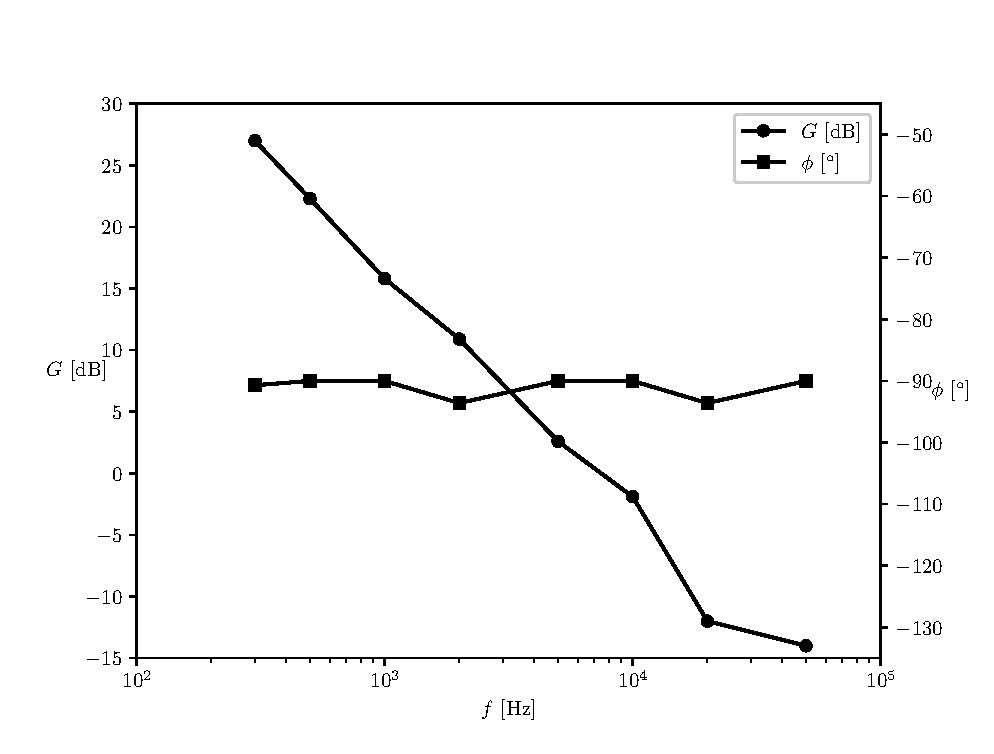
\includegraphics[width=0.8\hsize]{img/intex-graph1.eps}
                \caption{基本積分回路の周波数特性}
                \label{fig:intex1}
            \end{figure}

            図より, 周波数が上がるにつれて回路の利得が下がっていることがわかる.
            また, 入力に対する出力の位相の遅れは常に約 -90$^\circ$である.

    \subsection{実用積分回路}
        基本積分回路では, \ref{sec:ex4}節からも明らかなように,
        周波数の減少とともに出力電圧が無限大に増加してしまう.
        これを防ぐために抵抗$R_s$を追加した実用積分回路(PI)を
        図\ref{fig:nice-int}に示す.
        今回は各素子の値を
        $R_1 = 10\rm{k\Omega}$,
        $R_s = 20\rm{k\Omega}$, $C = 0.0022\rm{\mu F}$とする.

        \begin{figure}[h]
            \centering
            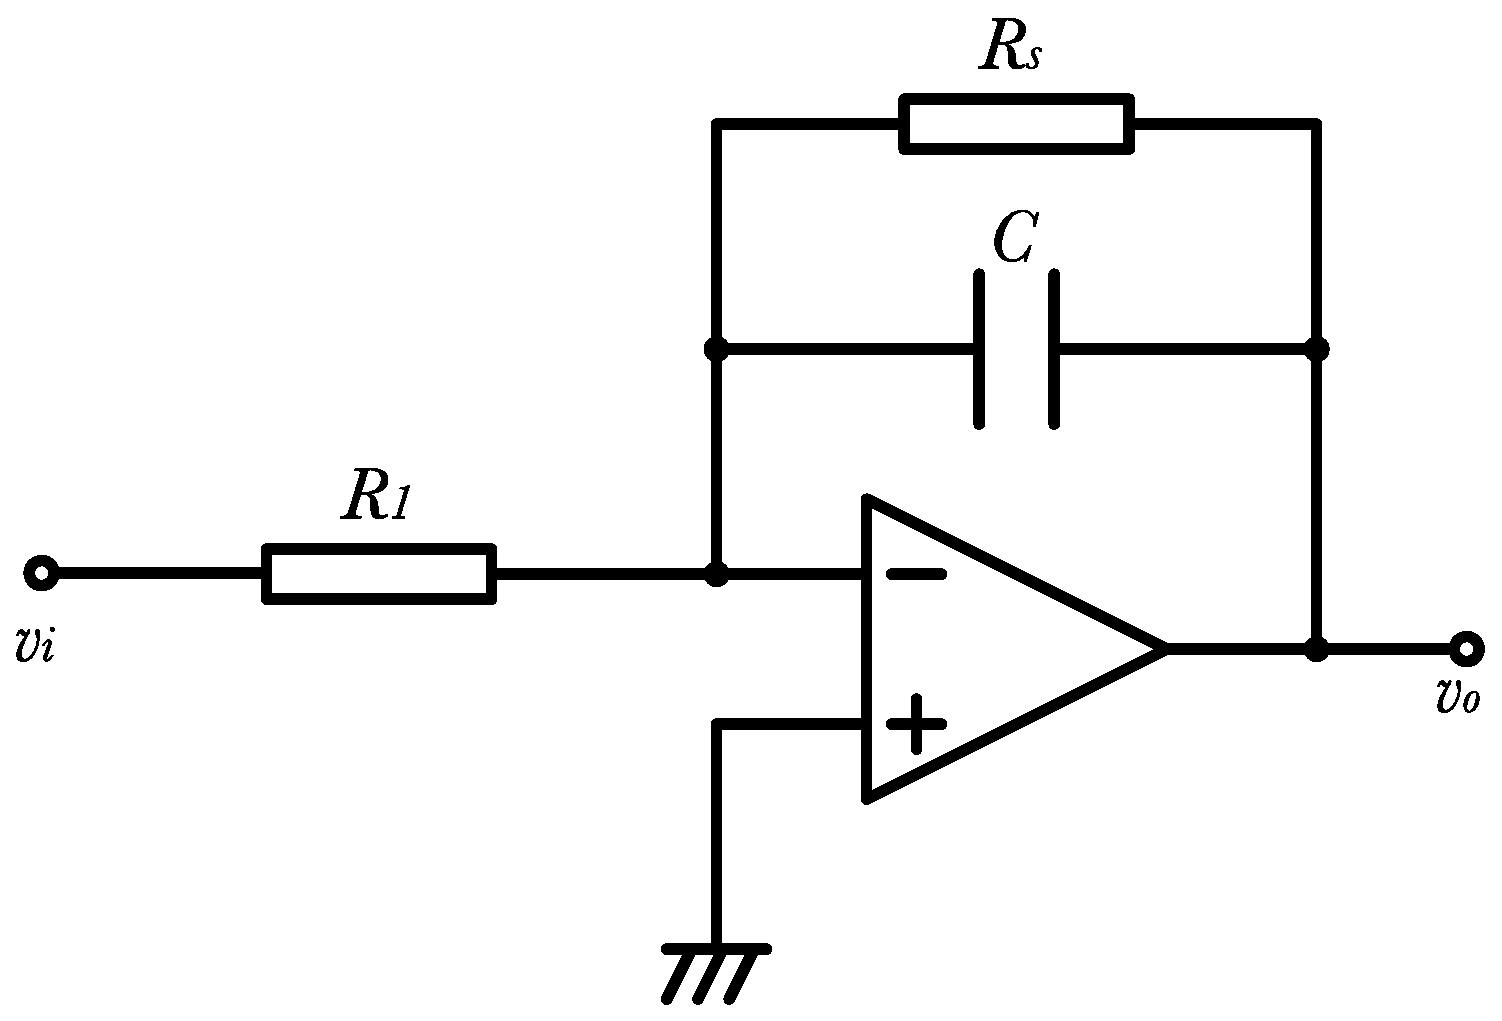
\includegraphics[width=0.7\hsize]{img/nice-int.eps}
            \caption{実用積分回路}
            \label{fig:nice-int}
        \end{figure}

        \subsection{周波数特性の測定} \label{sec:ex5}
            \ref{sec:ex4}と同様に振幅0.5V,
            周波数100Hz〜50kHzの正弦波を入力して周波数特性を測定する.
            表\ref{tab:nice-int}に計算結果を示す.

            \begin{table}[h]
                \caption{各周波数に対する出力波形の振幅と, 入力に対する遅れ}
                \label{tab:nice-int}
                \centering
                \begin{tabular}{r|rr|rr||r|rr|rr}
                    $f \ [\rm{kHz}]$ & $V_o \ [\rm{V]}$ & $G \ [\rm{dB}]$ & $t \ [\mu\rm{s}]$ & $\phi \ [^\circ]$ & $f \ [\rm{kHz}]$ & $V_o \ [\rm{V]}$ & $G \ [\rm{dB}]$ & $t \ [\mu\rm{s}]$ & $\phi \ [^\circ]$ \\ \hline \hline
                    0.1 & 2.0 & 6.0 & 5000 & -180.0 & 4 & 1.4 & 2.9 & 95 & -136.8 \\
                    0.5 & 2.0 & 6.0 & 1000 & -180.0 & 5 & 1.2 & 1.6 & 74 & -133.2 \\
                    1 & 2.0 & 6.0 & 460 & -165.6 & 10 & 0.7 & -3.1 & 30 & -108.0 \\
                    2 & 1.8 & 5.1 & 210 & -151.2 & 20 & 0.4 & -8.4 & 14 & -100.8 \\
                    3 & 1.6 & 4.1 & 130 & -140.4 & 50 & 0.1 & -20.0 & 5 & -90.0 \\
                \end{tabular}
            \end{table}

            表のデータをプロットしたものを図\ref{fig:nice-int-graph},
            表\ref{tab:int}, \ref{tab:nice-int}のデータを合わせてプロットしたものを
            図\ref{fig:int-com-graph}に示す.

            \begin{figure}[h]
                \centering
                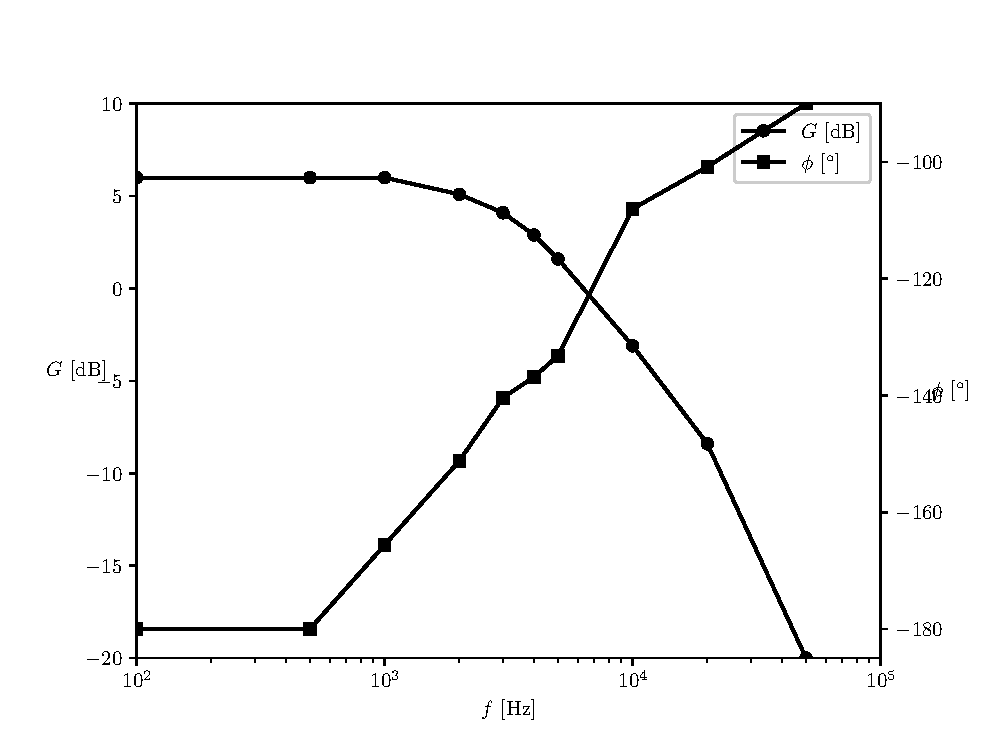
\includegraphics[width=0.8\hsize]{img/nice-int-graph.eps}
                \caption{実用積分回路の周波数特性}
                \label{fig:nice-int-graph}
            \end{figure}

            \begin{figure}[h]
                \begin{minipage}{0.5\hsize}
                    \centering
                    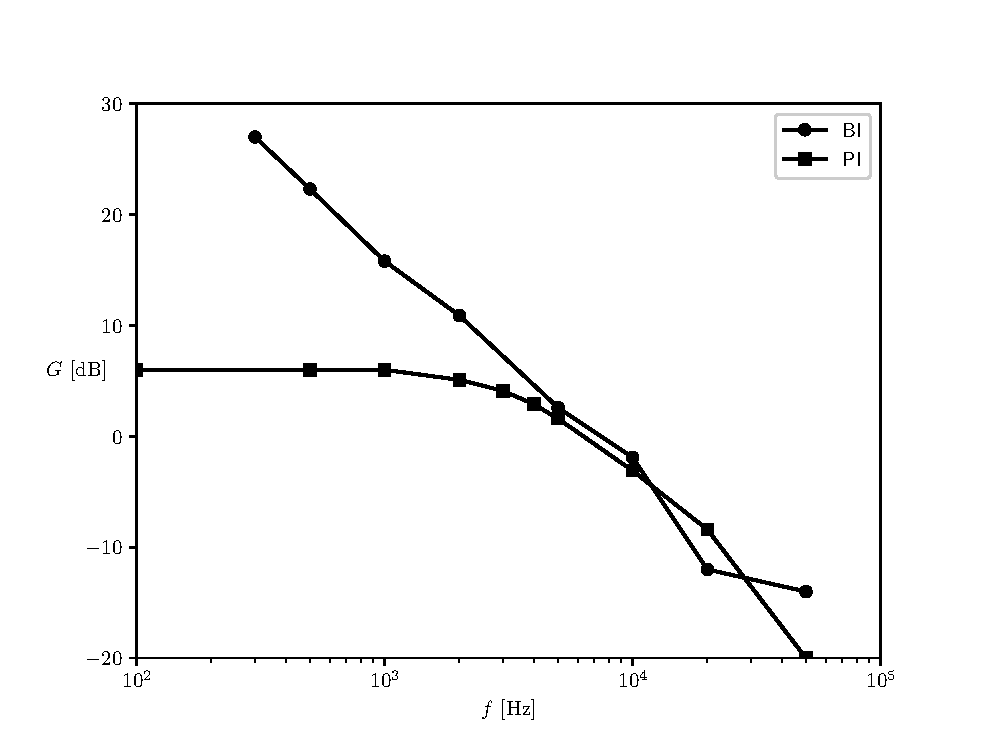
\includegraphics[width=1.1\hsize]{img/int-com-graph1.eps}
                \end{minipage}
                \begin{minipage}{0.5\hsize}
                    \centering
                    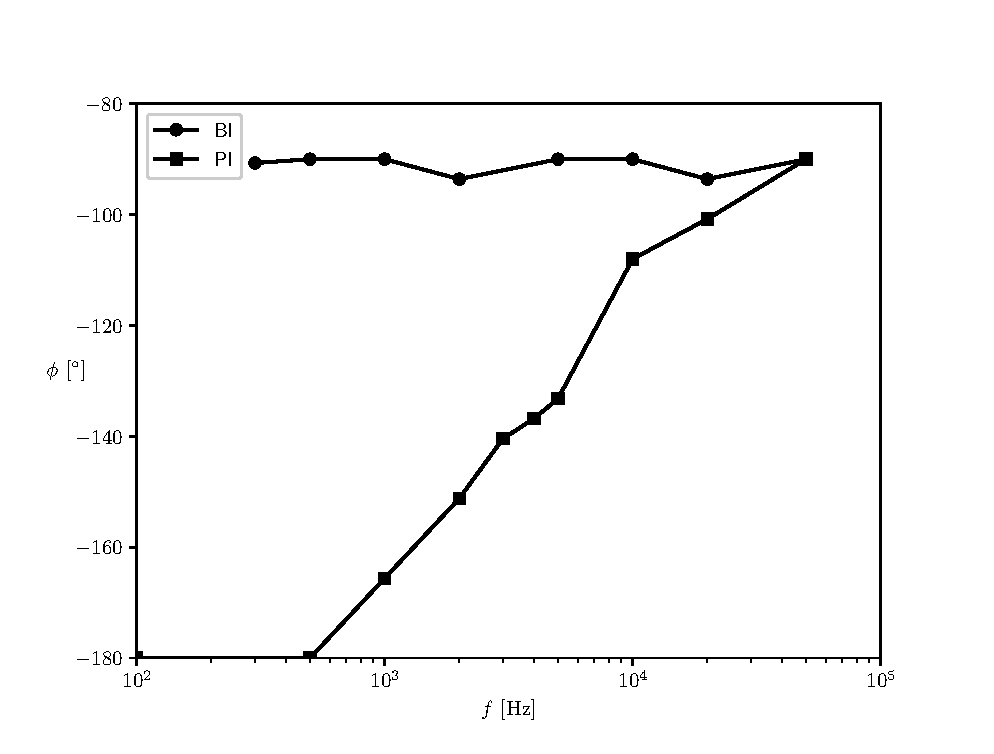
\includegraphics[width=1.1\hsize]{img/int-com-graph2.eps}
                \end{minipage}
                \caption{周波数特性の比較}
                \label{fig:int-com-graph}
            \end{figure}

            図より, 基本積分回路では周波数の減少につれて
            出力が上昇しているが,
            実用積分回路では一定値に収束している.
            また, それに伴い出力の位相も遅れていることがわかる.

    \subsection{課題3}
        \paragraph{実用積分回路の閉ループ利得と位相差を周波数の関数として具体的に求めよ. \\}
        図\ref{fig:nice-int}より,
        次の式を立てられる.

        \begin{numcases}
            {}
            v_i(t) = \{i_R(t) + i_C(t)\}R_1 & \nonumber \\
            v_o(t) = -i_R(t)R_s = ji_C(t)\frac{1}{\omega C} & \nonumber
        \end{numcases}

        これらをラプラス変換して,

        \begin{numcases}
            {}
            V_i(s) = \{I_R(s) + I_C(s)\}R_1 & \nonumber \\
            V_o(s) = -I_R(s)R_s = -\frac{I_C(s)}{sC} & \nonumber
        \end{numcases}

        となる. よって$v_i$から$v_o$の伝達関数は,

        \begin{equation*}
            \frac{V_i(s)}{V_o(s)} = -\frac{1}{\frac{R_s}{R_1} + sR_sC} = -\frac{R_1}{R_s + sR_1R_sC}
        \end{equation*}

        である. これに, $R_1 = 10\rm{k\Omega}$,
        $R_s = 20\rm{k\Omega}$, $C = 0.0022\rm{\mu F}$
        を代入すると, $\displaystyle -\frac{1}{0.000044s + 2}$となる.
        これに$s = j\omega$を代入すると
        $\displaystyle -\frac{1}{2 + j0.000044\omega} = -\frac{1}{2 + j0.000088\pi f}$
        となり, 閉ループ利得を表す周波数の関数となる.

        また, これの偏角を求めると,
        $\displaystyle\phi = \arctan\frac{0.000088\pi f}{2} = \arctan (0.000044\pi f)$
        となる.

        これらの式を\ref{sec:ex5}の結果に重ねてプロットしたものを
        図\ref{fig:intex2}に示す.

        \begin{figure}[h]
            \begin{minipage}{0.5\hsize}
                \centering
                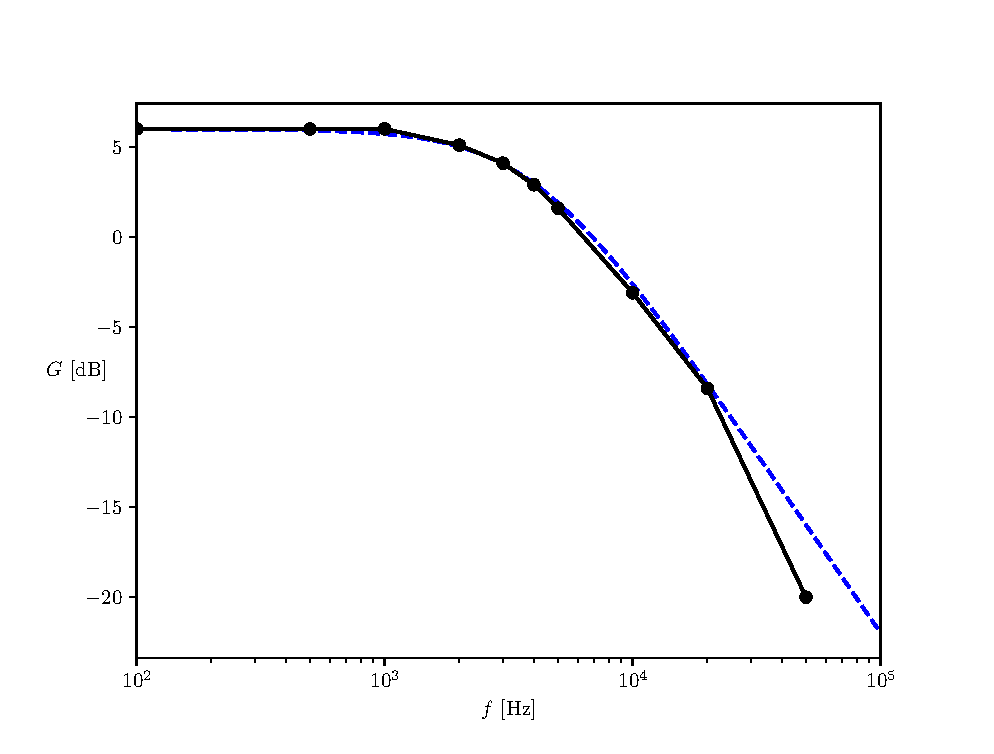
\includegraphics[width=1.1\hsize]{img/intex2-1.eps}
            \end{minipage}
            \begin{minipage}{0.5\hsize}
                \centering
                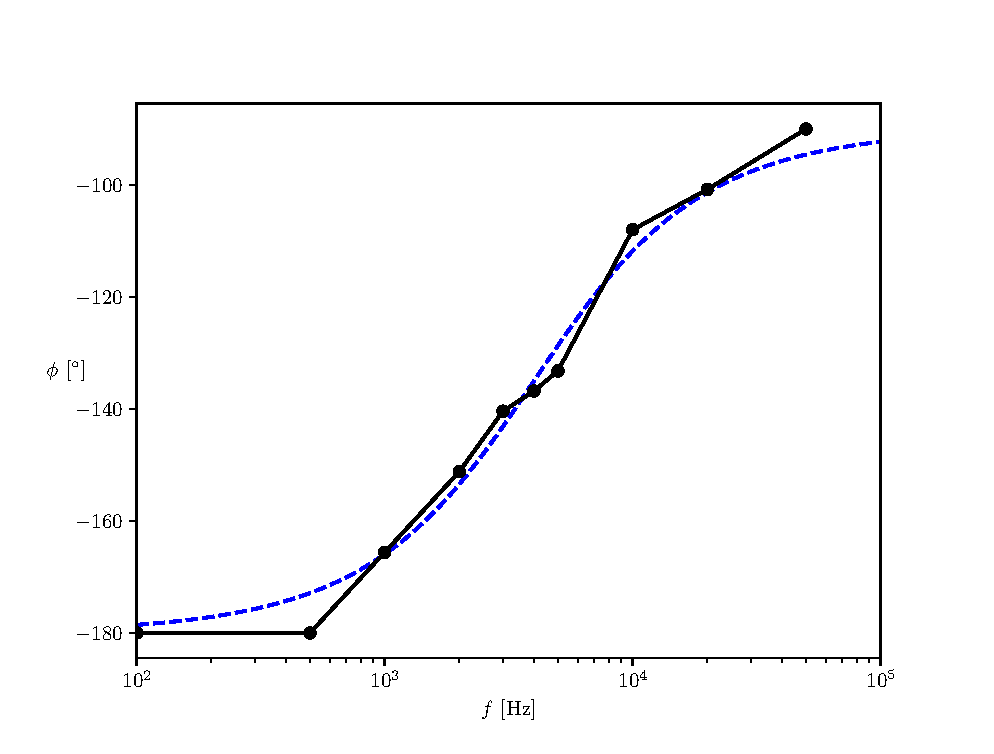
\includegraphics[width=1.1\hsize]{img/intex2-2.eps}
            \end{minipage}
            \caption{理論値と計測値の比較}
            \label{fig:intex2}
        \end{figure}
        
        実験が正しく行われていたことがわかる.

\section{フィルタ回路}
    フィルタ回路は信号の特定の周波数成分を取り出すための演算回路である.
    各種フィルタ回路についての説明は,
    実験テキスト\cite{text}に載っているため省略する.
    今回は1次のバンドパスフィルタについて実験を行う.
    図\ref{fig:band}に1次のバンドパスフィルタを示す.
    今回は各素子の値を
    $R_1 = R_2 = 10\rm{k\Omega}$,
    $C_1 = 0.01\rm{\mu F}$,
    $C_2 = 0.001\rm{\mu F}$とする.

    \begin{figure}[h]
        \centering
        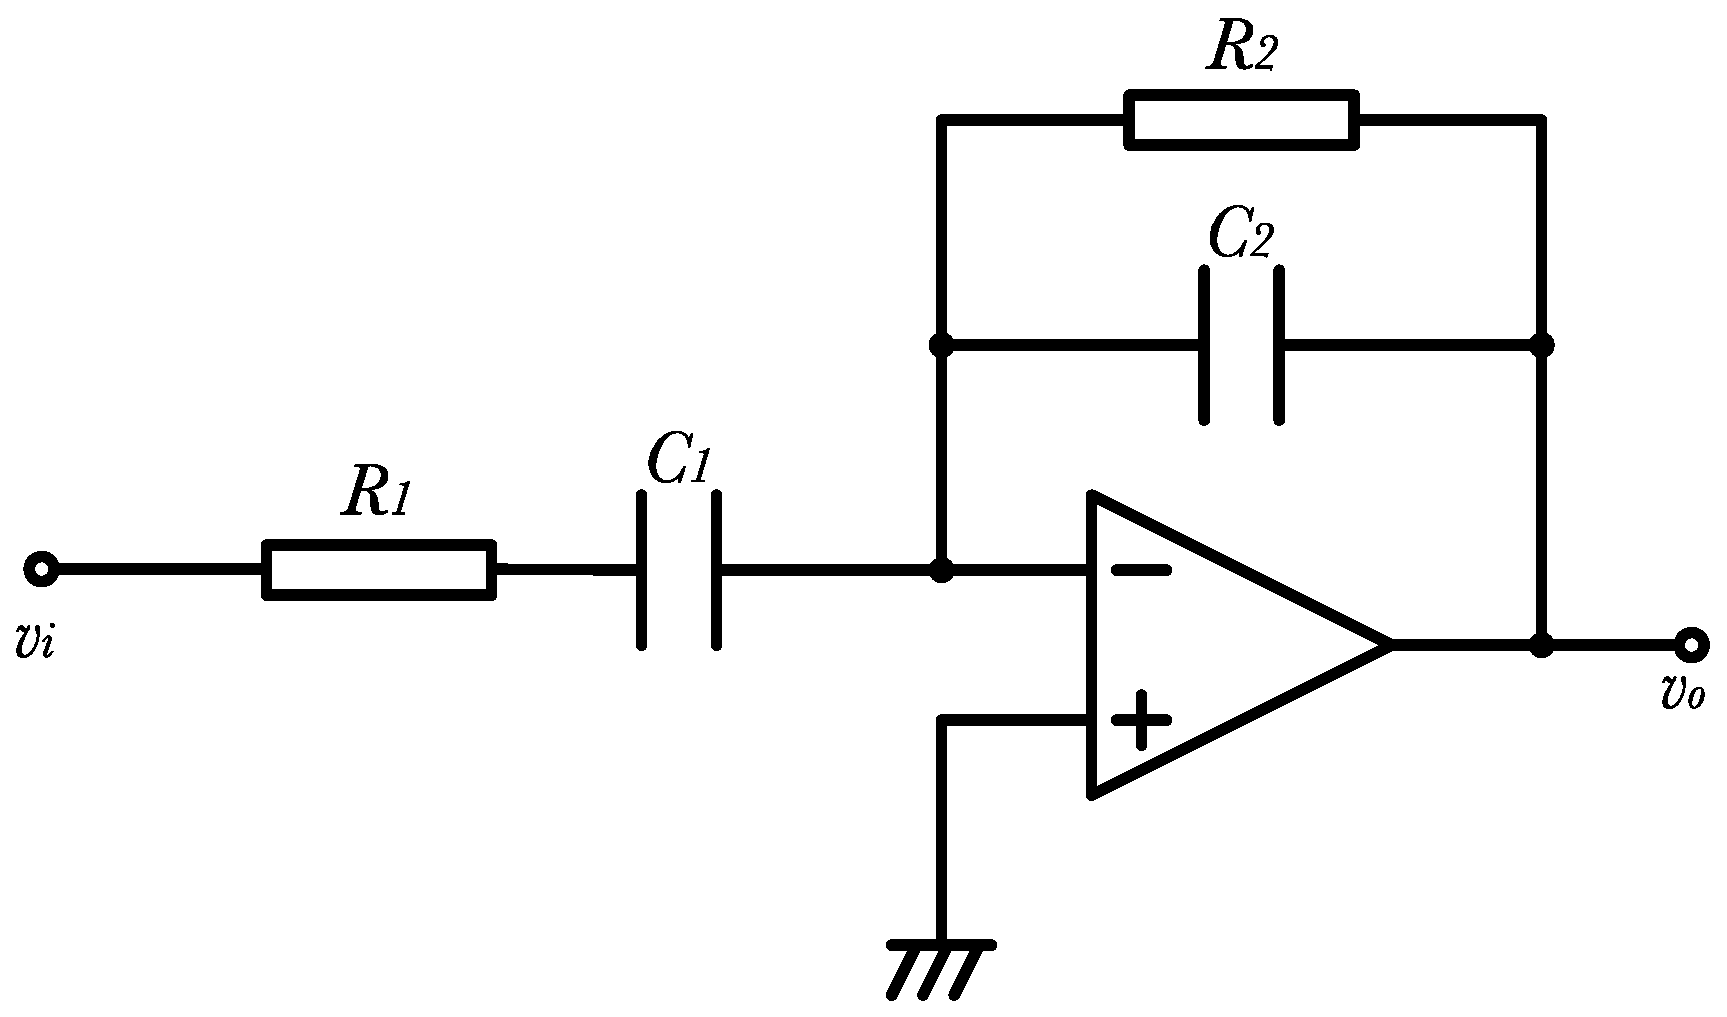
\includegraphics[width=0.7\hsize]{img/band.eps}
        \caption{1次のバンドパスフィルタ}
        \label{fig:band}
    \end{figure}

    この回路は実用微分回路と実用積分回路を組み合わせたもので,
    $\displaystyle\frac{1}{2\pi R_1C_1} < f < \frac{1}{2\pi R_2C_2}$
    の周波数帯の信号を取り出すことができる.
    また, この回路の周波数伝達関数は次のようになる.

    \begin{eqnarray}
        \frac{V_o}{V_i} &=& -\frac{1}{\left(R_1-j\frac{1}{\omega C_1}\right)\left(\frac{1}{R_2}+j\omega C_2\right)} = -\frac{j\omega}{-10^{-5}\omega^2 + j1.1\omega + 10^{4}} \label{equ:band1} \\
        \phi &=& \arctan\frac{1}{\omega C_1R_1}-\arctan (\omega C_2R_2) + \pi \label{equ:band2}
    \end{eqnarray}

    これらの式の導出は例によって実験テキスト\cite{text}を参考にされたい.

    \subsection{周波数特性の測定}
        
        回路の周波数特性を調べる.
        入力は振幅0.5V,
        周波数100Hz〜500kHzとする.
        測定結果を表\ref{tab:band}に示す.

        \begin{table}[h]
            \caption{各周波数に対する出力波形の振幅と, 入力に対する遅れ}
            \label{tab:band}
            \centering
            \begin{tabular}{r|rr|rr||r|rr|rr}
                $f \ [\rm{kHz}]$ & $V_o \ [\rm{mV]}$ & $G \ [\rm{dB}]$ & $t \ [\mu\rm{s}]$ & $\phi \ [^\circ]$ & $f \ [\rm{kHz}]$ & $V_o \ [\rm{mV]}$ & $G \ [\rm{dB}]$ & $t \ [\mu\rm{s}]$ & $\phi \ [^\circ]$ \\ \hline \hline
                0.1 & 60 & -24.4 & 2500 & 90.0 & 10 & 800 & -1.9 & 55 & -18.0 \\
                0.2 & 130 & -17.7 & 1500 & 72.0 & 12 & 760 & -2.4 & 38 & -15.8 \\
                0.5 & 300 & -10.5 & 600 & 72.0 & 14 & 700 & -3.1 & 30 & -28.8 \\
                1 & 520 & -5.7 & 350 & 54.0 & 16 & 680 & -3.3 & 25 & -36.0 \\
                1.2 & 600 & -4.4 & 300 & 50.4 & 18 & 610 & -4.3 & 22 & -37.7 \\
                1.4 & 680 & -3.3 & 260 & 49.0 & 20 & 600 & -4.4 & 18 & -50.4 \\
                1.6 & 700 & -3.1 & 250 & 36.0 & 50 & 300 & -10.5 & 6.3 & -66.6 \\
                1.8 & 720 & -2.9 & 240 & 24.5 & 100 & 180 & -14.9 & 3.0 & -72.0 \\
                2 & 760 & -2.4 & 210 & 28.8 & 200 & 80 & -21.9 & 1.3 & -86.4 \\
                5 & 800 & -1.9 & 100 & 0 & 500 & 40 & -29.1 & 0.50 & -90.0 \\
            \end{tabular}
        \end{table}

        表のデータと式\ref{equ:band1}, \ref{equ:band2}を重ねてプロットしたものを図\ref{fig:bandex}に示す.

        \begin{figure}[h]
            \begin{minipage}{0.5\hsize}
                \centering
                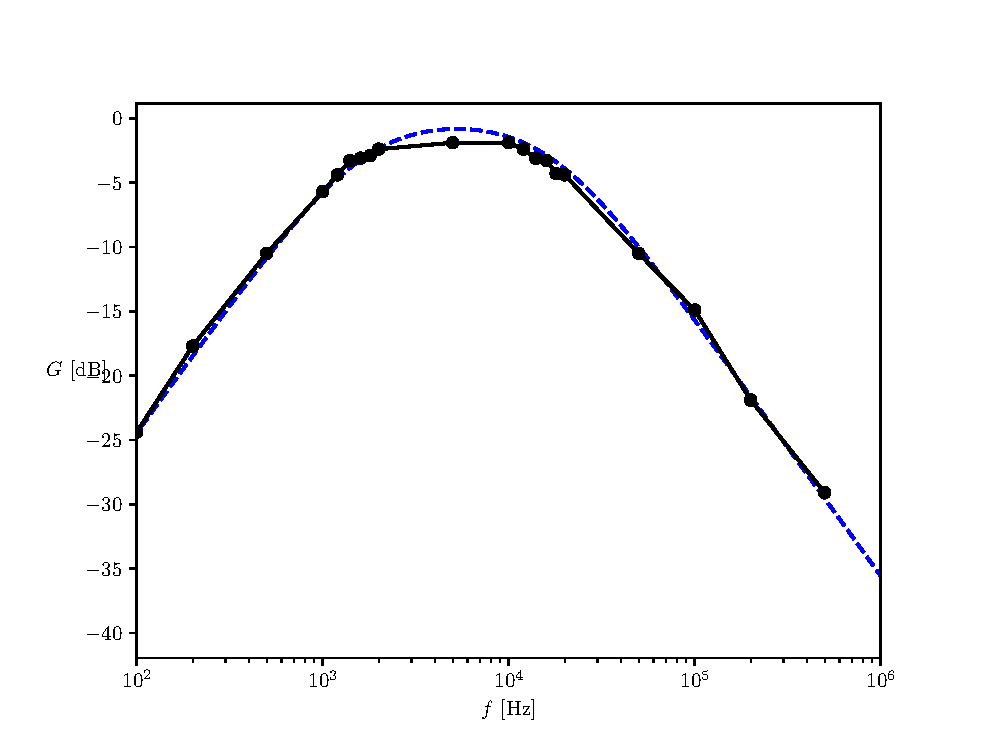
\includegraphics[width=1.1\hsize]{img/band-1.eps}
            \end{minipage}
            \begin{minipage}{0.5\hsize}
                \centering
                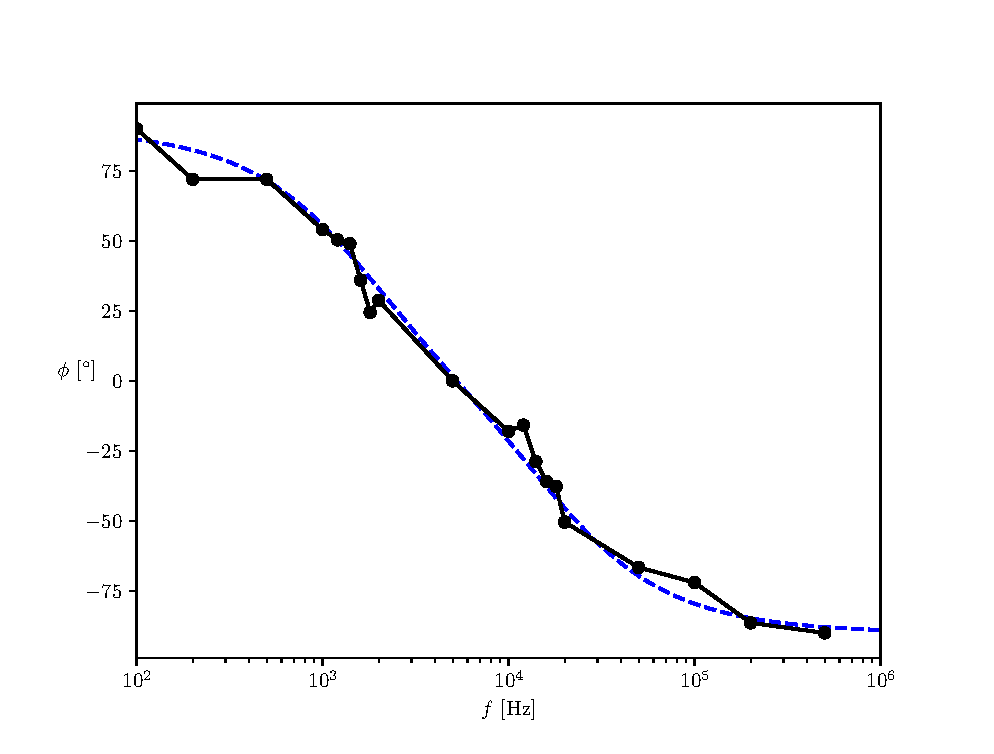
\includegraphics[width=1.1\hsize]{img/band-2.eps}
            \end{minipage}
            \caption{理論値と計測値の比較}
            \label{fig:bandex}
        \end{figure}

        図より, 理論通りにバンドパスフィルタとして機能していることがわかる.
        また, 位相線図の誤差が低周波数側と高周波数側で対称的なのは,
        OPアンプの動作のためであると考えられる.
    
\begin{thebibliography}{99}
    \bibitem{text} OPアンプの基礎・応用, 電子制御工学実験$\cdot$ 4年後期テキスト, 2020
\end{thebibliography}
\end{document}